\documentclass[article]{standalone}
\usepackage[subpreambles=false]{standalone}
\usepackage{preamble}
\usepackage{import}
\usepackage{graphicx,subfigure}


\begin{document}
\section{Schematic Diagrams}\label{sec:schematics}
These are listed at the end.

\begin{figure}
\centering
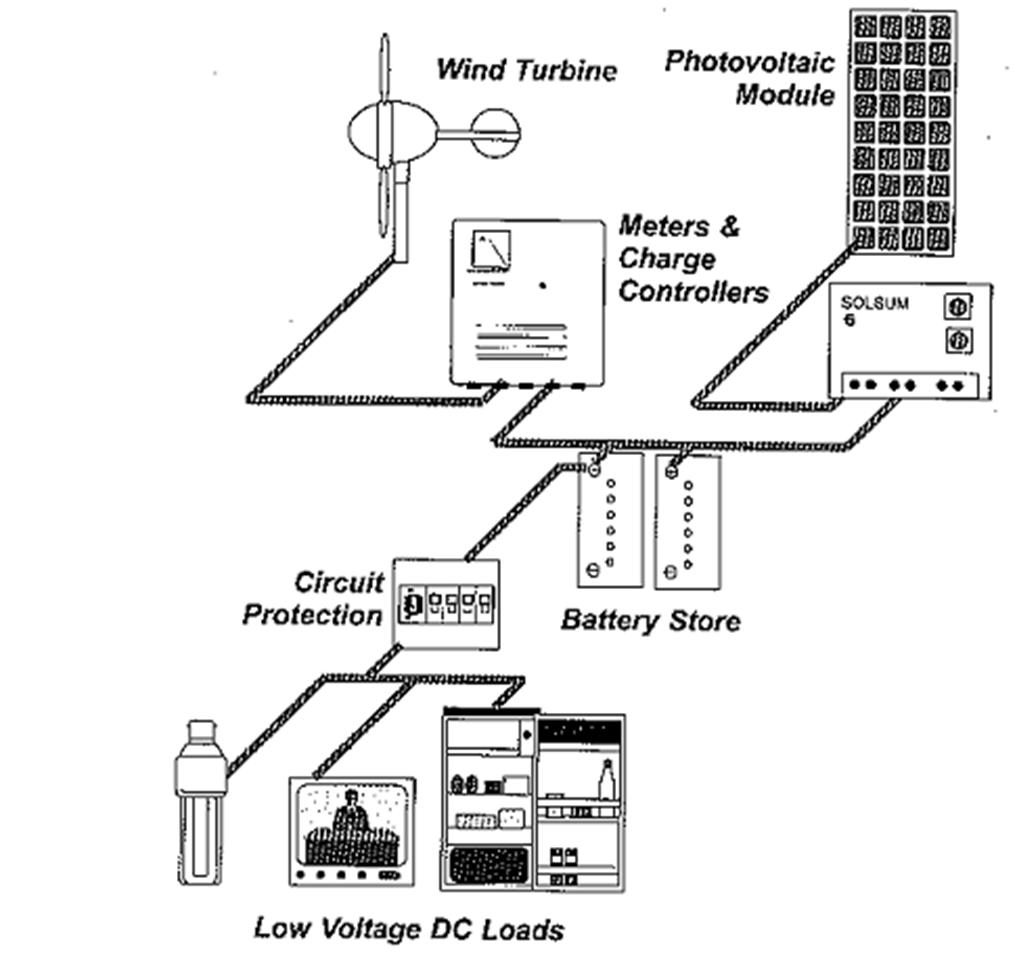
\includegraphics[width=0.9\linewidth]{../figures/solarwindDC.jpg}
\caption{Example schematic showing the main components of an off-grid domestic solar PV and wind system for DC loads}
\label{fig:solarwindDC}
\end{figure}


\begin{figure}
\centering
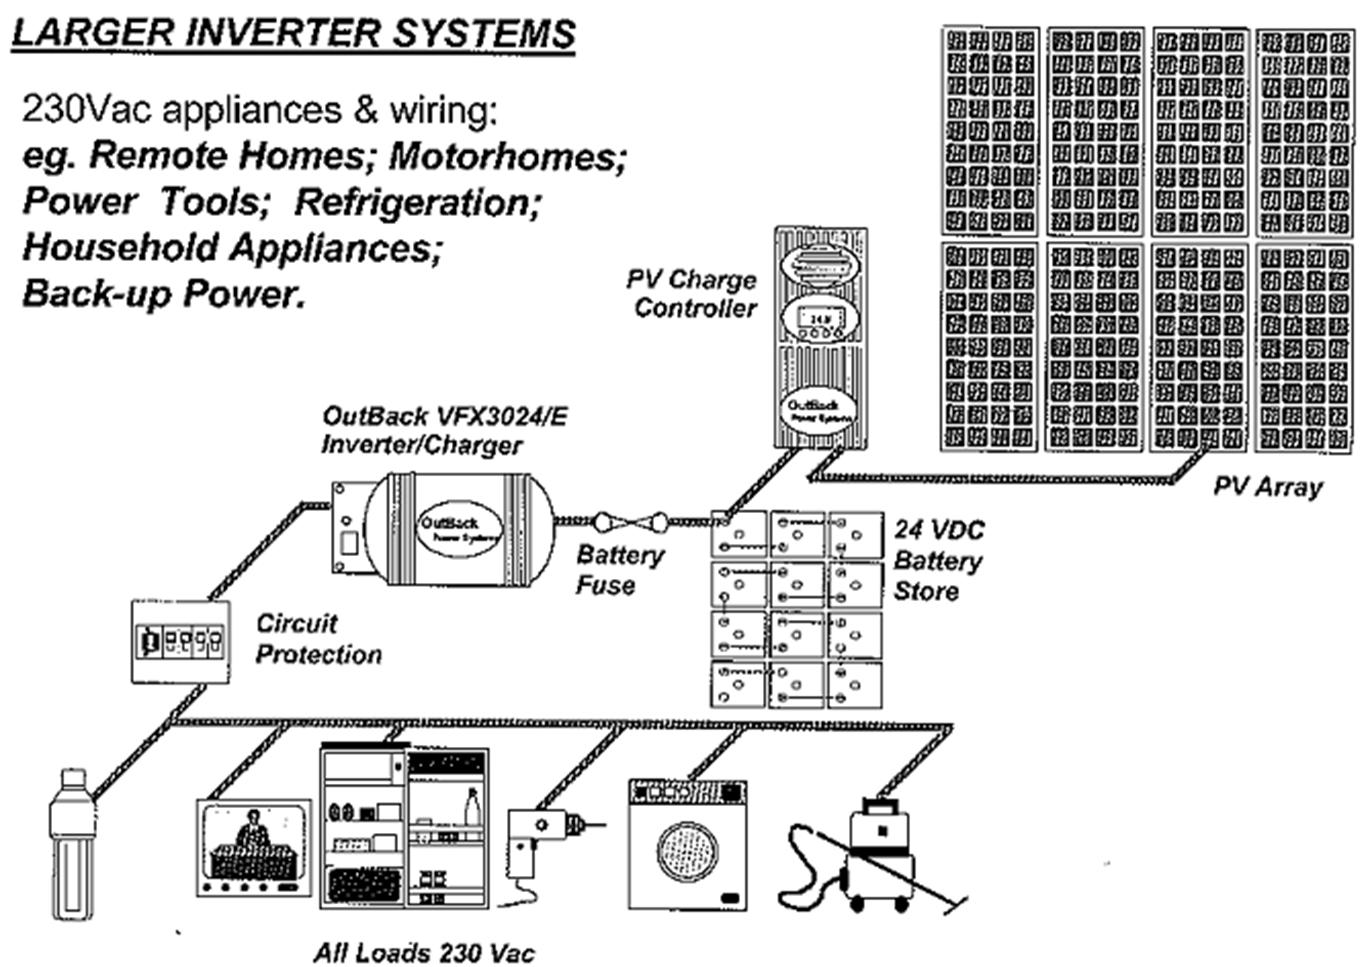
\includegraphics[width=0.9\linewidth]{../figures/large-off-grid-solar-PV-AC.jpg}
\caption{Example schematic showing the main components of an off-grid domestic solar PV system for AC loads}
\label{fig:solarAC}
\end{figure}


\begin{figure}
\centering
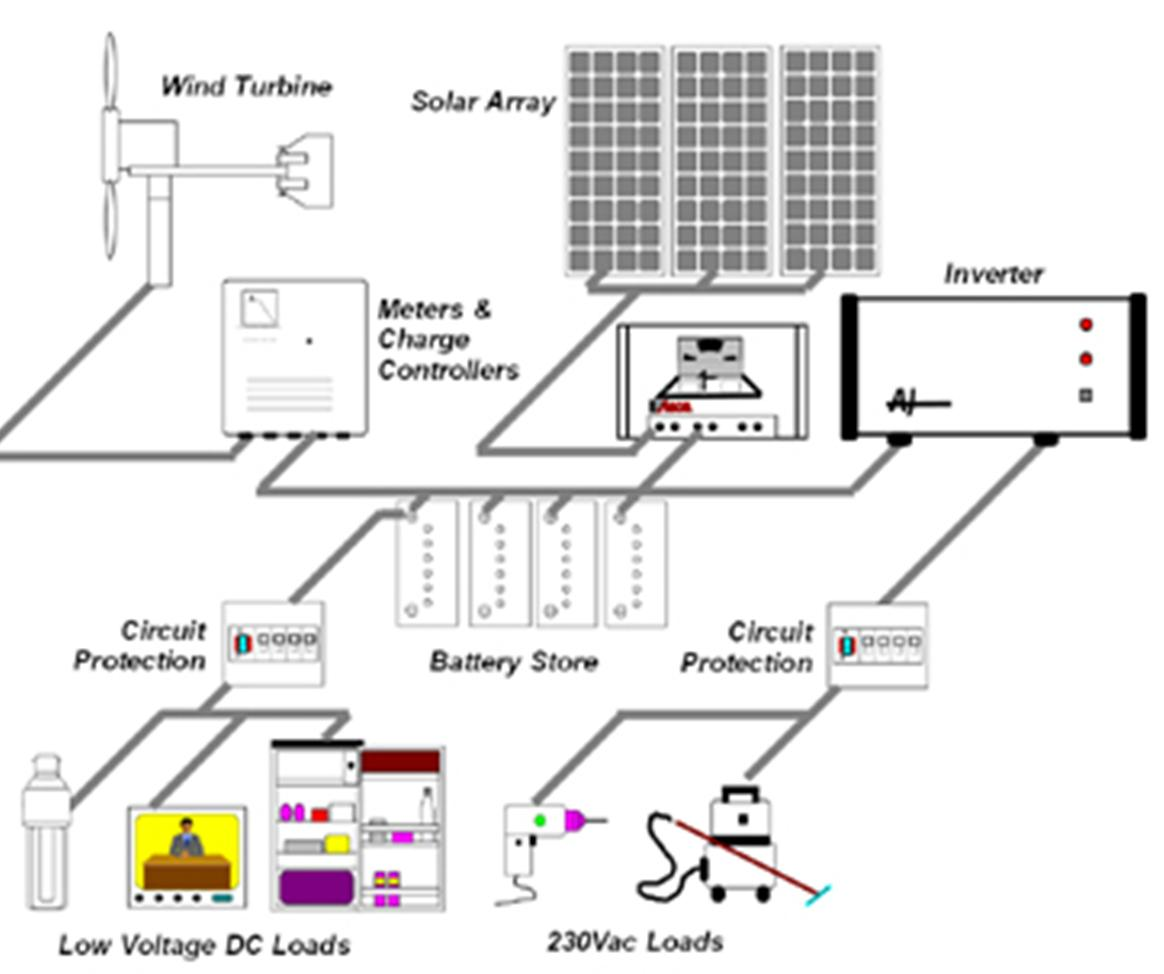
\includegraphics[width=0.9\linewidth]{../figures/large-off-grid-solarwind-ACDC.jpg}
\caption{Example schematic showing the main components of a combined off-grid domestic solar PV and wind system for AC and DC loads}
\label{fig:solarwindACDC}
\end{figure}


\begin{figure}
\centering
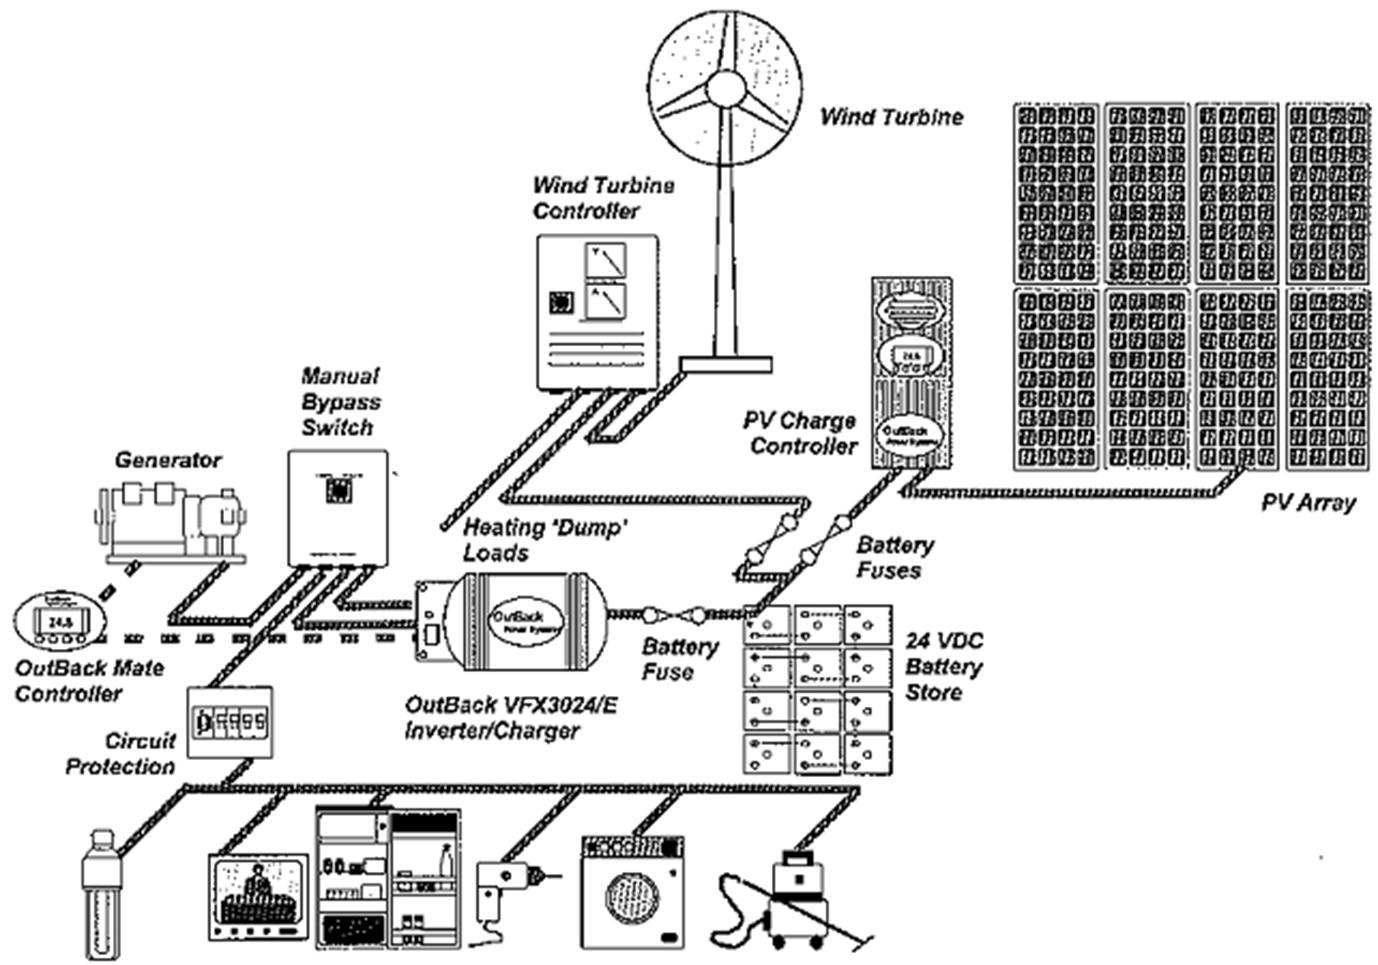
\includegraphics[width=0.9\linewidth]{../figures/large-off-grid-solarwind-gen-ACDC.jpg}
\caption{Example schematic showing the main components of an off-grid domestic solar PV and wind system for AC and DC loads, with generator backup}
\label{fig:solarwindACDCgen}
\end{figure}
\end{document}